\section{The CGIO Software Library}
\label{s:library}
\thispagestyle{plain}

\subsection{Node - The Building Block}
\label{s:nodebb}

A database is a hierarchical system that is built around
the concept of a "node".
Each node contains information about itself and its ancestors and
possibly data (e.g., arrays, vectors, character strings, etc.).
Each of these nodes, in turn, may be connected to an arbitrary number of
children, each of which is itself a node.
In this system, a node contains user-accessible information related
to identification, name, type, and amount of data associated with it,
and pointers to child nodes.
Basic nodal information includes:

\begin{itemize}
\item a unique ID (node locator)
\item a name (character string) used to describe the node and its data
\item a label (character string) an additional field used to describe the
      node and its data.
      It is analogous to, but not exactly the same as, the name.
\item information describing the type and amount of data
\item data
\item IDs of child nodes
\end{itemize}

There are no restrictions on the number of child nodes that a node can
have associated with it in the database.
This structure allows the construction of a hierarchical database as
shown in \autoref{f:example} on p.~\pageref*{f:example}.
As illustrated in the figure, it is possible to reference nodes in a
second file (\textit{File\_Two}) from the original file
(\textit{File\_One}).
This is the concept of ``linking.''
\begin{figure}[!htb]
   \centering
   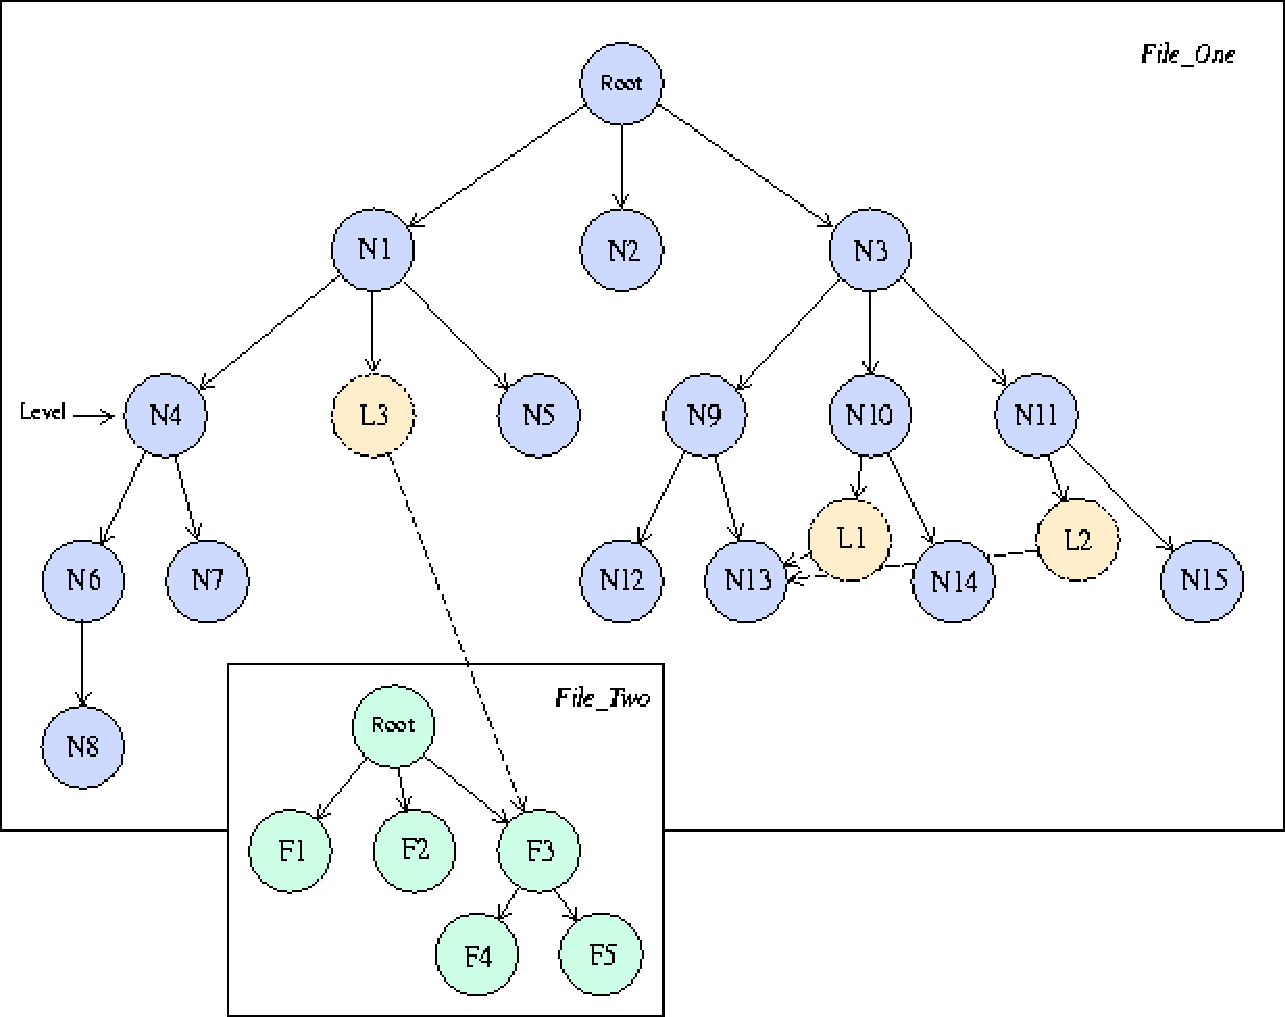
\includegraphics[width=6.0in]{figure}
   \caption{Example Database Hierarchy of Nodes}
   \label{f:example}
\end{figure}

A node knows about itself and its children, but it does not know
anything about its parent.
This means that it is possible to traverse ``down'' the tree by making
queries about what lies below the current node, but it is not possible
to traverse ``up'' the tree by making queries about nodes above a given
node.
If it is desired to move back up the tree, the user must keep track of
that information.

All database files start with a root node, which is created automatically
when a new file is opened.
There is only one root node in a database file, and may be referenced
by the database Root ID or by name as ``\key{/}''.

\subsection{Node Attributes}
\label{s:attributes}

Each node in the database may have zero to many subnodes that are
associated with it, as well as its own data.
The following are a list of attributes accessible by the user for a node
in the hierarchical database system.

\begin{Ventryi}{Number of Dimensions}
\item [Data]
      The data associated with a node.
\item [Data Type]
      A 2-byte character field, blank filled, case sensitive.
      Specifies the type of data (e.g., real, integer, character)
      associated with this node.
      The supported data types are listed in \autoref{t:datatype}
      on p.~\pageref*{t:datatype}.
\item [Dimensions]
      An integer vector containing the number of elements within
      each dimension.
      For example, if the array \fort{A} was declared (using Fortran) as
      \fort{A(10,20)}, the Dimension vector would contain two entries
      (10,20).
\item [ID]
      A unique identifier to access a given node within a file.
      This field contains sufficient information for the database manager
      to locate the node within a file.
      For any given node, the ID is generated only after the file it
      resides in has been opened by a program and the user requests
      information about the node.
      The ID is valid only within the program that opened the file and
      while that file is open.
      If the file is closed and reopened, the ID for any given node
      may be different.
      Within different programs, the node ID for the same node may
      also be different.
      The ID is never actually written into a file.
\item [Label]
      A 32-byte character field.
      The rules for Labels are identical to those for Names.
      Unlike names, Labels do not have to be unique.
      The Label field was introduced to allow ``data typing'' similar to
      the ``typedef'' concept in C.
      Using the Label field in this way allows programs to know some
      additional information about the use of the node itself or its
      child nodes and to call specific subroutines to read the data or
      react in specific ways upon detection of the type.
\item [Name]
      A 32-byte character field.
      The names of child nodes directly attached to a parent node must
      be unique.
      For example, in \autoref{f:example}, all nodes directly attached
      to N3 must have unique names.
      When a request to create a new node is made, the databse manager
      checks the requested name against the other names of the child
      nodes of the specified parent.
      If the requested name is not unique, an error is returned.

      Legal characteristics of a name are a A-Z, a-z, 0-9, and special
      characters (ASCII values from 32 to 126, except for the forward
      slash ``/'' (ASCII number 47)).
      Names will be blank filled to 32 bytes; they are case sensitive.
      Leading blanks are discarded and trailing blanks are ignored,
      whereas internal blanks are significant.

      \emph{Note}: Names passed from C must have the null
      ``\textbackslash0'' character appended to them.
      Names returned through the C interface will have the
      null character appended to them.
      Therefore, C programs should allocate 33 bytes for any Name in
      order to accommodate the null character.

      Fortran programs can allocate 32 characters for Names.
      The Fortran interface takes care of adding or removing the null
      character as required.
\item [Names of Subnodes]
      A list of names of the subnodes (children) of a node.
      (This is the information contained in the child table.)
\item [Number of Dimensions]
      The dimensionality of the data.
      ADF views all data as an array and can handle from zero (i.e., no
      data) to 12 dimensions.
      A ``0'' is used if the data type is empty.
      Thus, a scalar is viewed as a vector with one dimension and
      length 1.
\item [Number of Subnodes]
      The number of child nodes directly attached to any given node.
      Each node can have zero or more child nodes directly associated
      with it.
\item [Pointer]
      An address, from the point of view of a programming language.
      Pointers are like jumps, leading from one part of the data
      structure to another.
\end{Ventryi}

\subsection{Supported Data Types}

\begin{longtable}{l >{\quad}l >{\quad}l >{\quad}l}
\caption[Data Types]{\textbf{Data Types}}
\label{t:datatype}
\\ \hline\hline \\*[-2ex]
\bold{Notation} & \bold{Data Type} & \bold{C Type} & \bold{Fortran Type}
\\*[1ex] \hline\hline \\*[-2ex]
\key{MT} & No Data                 &  & \\
\key{I4} & 32-bit Integer          &  \key{int} & \fort{integer*4} \\
\key{I8} & 64-bit Integer          &  \key{cglong\_t} & \fort{integer*8}\\
\key{U4} & 32-bit Unsigned Integer &  \key{unsigned int} & \fort{integer*4} \\
\key{U8} & 64-bit Unsigned Integer &  \key{cgulong\_t} & \fort{integer*8} \\
\key{R4} & 32-bit Real             &  \key{float} & \fort{real*4} \\
\key{R8} & 64-bit Real             &  \key{double} & \fort{real*8} \\
\key{C1} & Character               &  \key{char} & \fort{character} \\
\key{B1} & Byte (unsigned byte)    &  \key{unsigned char} & \fort{character*1} \\
\key{LK} & Link                    &  &
\\*[1ex] \hline\hline
\end{longtable}

The \key{MT} node contains no data, and is typically used as a
container for subnodes (children).

A link is denoted by \key{LK}, and defines the
linkage between nodes and subnodes. A link provides a mechanism for
referring to a node that physically resides in a different part of the
hierarchy or a different database file. The link parallels a soft link
in the UNIX operating system in that it does not guarantee that the
referenced node exists. The database manager will ``resolve'' the link
only when information is requested about the linked node or it's children.

\subsection{Glossary of Terms}
\label{s:glossary}

\begin{Ventryi}{Node Name}
\item [Child]
      One of the subnodes of a Parent.
      A child node does not have knowledge of its parent node.
      The user must keep track of this relationship.
\item [Database]
      The representation of a hierarchy of nodes on disk files.
      By use of links, it may physically span multiple files.
\item [File]
      An database file, which a single root node and its underlying structure.
\item [ID]
      A unique identifier to access a given node within a database file.
      This field contains sufficient information for the database manager
      to locate the node within a file.
      For any given node, the ID is generated only after the file it
      resides in has been opened by a program and the user requests
      information about the node.
      The ID is valid only within the program that opened the file and
      while that file is open.
      If the file is closed and reopened, the ID for any given node
      may be different. Within different programs, the node-ID for the
      same node may also be different.
      The ID is never actually written into a file.
\item [Link-Node]
      A special type of node.
      Links are created using the
      \texttt{cgio\_create\_link} (\autoref{create_link})
      subroutine.
      The data type of this node is \key{LK}, and its data is a
      one-dimensional array containing the name of the file (if other
      than the current file) containing the node to be linked and the
      full path name in that file from the root node to the desired
      node.

      Links provide a mechanism for referring to a node that physically
      resides in a different part of the hierarchy.
      The node pointed to by a link may or may not reside in the same
      file as the link itself.
      A link within ADF is very similar to a ``soft'' link in the
      UNIX operating system in that it does not guarantee that the
      referenced node exists.
      ADF will ``resolve'' the link only when information is requested
      about the node.
      If the ID of a link-node is used in an ADF call, the effect of
      the call is the same as if the ID of the linked-to node was used.
      Note that a link node does not have children itself.
      In \autoref{f:example} on p.~\pageref*{f:example}, the children
      seen for \key{L3} are \key{F4} and \key{F5}.
      If a child is ``added'' to \key{L3}, then in reality, the child
      is added to \key{F3}.
      There are specialized subroutines provided to create link nodes
      and extract the link details.
\item [Node]
      The single component used to construct a database.
\item [Node name]
      A node has a 32-character name.
      Every child node directly under a given parent must have a unique
      name.
      Legal characteristics in a name are \key{A-Z}, \key{a-z},
      \key{0-9}, and special characters (ASCII values from 32 to
      126, omitting the forward slash ``\key{/}'', ASCII number 47).
      Names will be blank filled to 32 bytes; they are case sensitive.
      Leading blanks are discarded and trailing blanks are ignored,
      whereas internal blanks are significant.
\item [Parent]
      A node that has subnodes directly associated with it.
\item [Pathname]
      Within a database, nodes can be referenced using the name of a node
      along with its parent ID, or by using a ``pathname'' whose syntax is
      roughly the same as a path name in the UNIX environment.
      A pathname that begins with a leading slash ``\key{/}'' is
      assumed to begin at the root node of the file.
      If no leading slash is given, the name is assumed to begin at the
      node specified by the parent ID.
      Although there is a 32-character limitation on the node Name,
      there is no restriction on the length of the pathname.
      For example, equivalent ways to refer to node \key{N8} in
      \autoref{f:example} are:
      \begin{itemize}
      \item Node-ID for \key{N6} and name = ``\key{N8}''
      \item Node-ID for \key{N4} and name = ``\key{N6/N8}''
      \item Node-ID for \key{N1} and name = ``\key{N4/N6/N8}''
      \item Node-ID for the \key{Root\_Node} and name =
            ``\key{/N1/N4/N6/N8}''
      \end{itemize}
\end{Ventryi}

\subsection{Conventions and Implementations}
\label{s:conventions}

\begin{Ventryi}{return codes}
\item [C]
      All input strings are to be null terminated.
      All returned strings will have the trailing blanks removed and
      will be null terminated.
      Variables declared to hold Names, Labels, and Data-Types should
      be at least 33 characters long.
      \textit{cgns\_io.h} has a number of variables defined.
      An example declaration would be:
\begin{indlefttt}
char name[CGIO\_MAX\_NAME\_LENGTH+1];
\end{indlefttt}
\item [Fortran]
      Strings will be determined using inherited length.
      Returned strings will be blank filled to the specified length.
      All returned names will be left justified and blank filled on the
      right.
      There will be no null character.
      An example declaration would be:
\begin{indlefttt}
PARAMETER CGIO\_MAX\_NAME\_LENGTH=32
CHARACTER*(CGIO\_MAX\_NAME\_LENGTH) NAME
\end{indlefttt}
      or include the Fortran header file \textit{cgns\_io\_f.h}
      which defines these parameters.
\item [ID]
      A unique identifier to access a given node within a database.
      For any given node, the ID is generated only after the file it
      resides in has been opened by a program and the user requests
      information about the node.
      The ID is valid only within the program that opened the file and
      while that file is open.
      If the file is closed and reopened, the ID for any given node
      may be different.
      Within different programs, the node ID for the same node may
      also be different.
      The ID is not ever actually written into a file.

      The declaration for variables that will hold node IDs should be
      for an 8-byte real number.
\item [Indexing]
      All indexing is Fortran-like in that the starting index is 1 and
      the last is \fort{N} for $N$ items in an index or array
      dimension.
      The array structure is assumed to be the same as in Fortran
      with the first array dimension varying the fastest and the last
      dimension varying the slowest.
 
      The index starting at one is used in
      \texttt{cgio\_read\_data} (\autoref{read_data}),
      \texttt{cgio\_write\_data} (\autoref{write_data}),
      \texttt{cgio\_children\_names} (\autoref{children_names}), and
      \texttt{cgio\_children\_ids} (\autoref{children_ids}).
 
      The user should be aware of the differences in array indexing
      between Fortran and C.
      The subroutines
      \texttt{cgio\_read\_all\_data} (\autoref{read_all_data}) and
      \texttt{cgio\_write\_all\_data} (\autoref{write_all_data})
      merely take a pointer to the beginning of the data, compute how
      much data is to be read/written, and process as many bytes as
      have been requested.
      Thus, these routines effectively make a copy of memory onto disk
      or vice versa.
      Given this convention, it is possible for a C program to
      use standard C conventions for array indexing and use
      \texttt{cgio\_write\_all\_data} to store the array on disk.
      Then a Fortran program might use \texttt{cgio\_read\_all\_data} to
      read the data set.
      Unless the user is aware of the structure of the data, it is
      possible for the array to be transposed relative to what is
      expected.
 
      The implications of the assumed array structure convention can be
      quite subtle.
      The subroutines \key{cgio\_write\_data} and
      \key{cgio\_read\_data} assume the Fortran array structure in
      order to index the data.
      Again, unless the user is aware of the implications of this, it
      is possible to write an array on disk and later try to change a
      portion of the data and not change the correct numbers.
 
      As long as users are aware of how their data structure maps onto
      the database, there will not be any problems.
\item [return codes]
      The CGIO routines return an integer code indicating whether they
      were successfull or not. On success, 0 (\key{CGIO\_ERR\_NONE}) is
      returned. A non-zero return indicates an error. Return codes < 0
      indicate an error at the CGIO level; codes > 0 indicate an
      error in the database manager. See \autoref{s:messages}
      for a list of error codes and mesages.
\end{Ventryi}

\subsection{Limits and Sizes}
\label{s:defaults}

The following default values, sizes, and limits are defined in the
header file \textit{cgns\_io.h}.

\begin{longtable}{l >{\quad}l >{\quad}l}
\caption[Default Values and Sizes]{\textbf{Default Values and Sizes}}
\label{t:defaults}
\\ \hline\hline \\*[-2ex]
\bold{Define} & \bold{Value} & \bold{Attribute}
\\*[1ex] \hline\hline \\*[-2ex]
\key{CGIO\_MAX\_DATATYPE\_LENGTH} & 2    & Data type length \\
\key{CGIO\_MAX\_DIMENSIONS}       & 12   & Maximum dimensions \\
\key{CGIO\_MAX\_NAME\_LENGTH}     & 32   & Name length \\
\key{CGIO\_MAX\_LABEL\_LENGTH}    & 32   & Label length \\
\key{CGIO\_MAX\_VERSION\_LENGTH}  & 32   & Version length \\
\key{CGIO\_MAX\_DATE\_LENGTH}     & 32   & Date length \\
\key{CGIO\_MAX\_ERROR\_LENGTH}    & 80   & Maximum length of error string \\
\key{CGIO\_MAX\_LINK\_DEPTH}      & 100  & Maximum link depth \\
\key{CGIO\_MAX\_FILE\_LENGTH}     & 1024 & File name length \\
\key{CGIO\_MAX\_LINK\_LENGTH}     & 4096 & Maximum link data size
\\*[1ex] \hline\hline\hline
\end{longtable}

